\subsection{Building avoidance}\label{s:testBuildingAvoidance}

\noindent \paragraph{Scenario:} The \emph{UAS}  is flying the mission given by (tab. \ref{tab:missionSetupForBuildingAvoidanceScenario}) in the \emph{open space environment}. There exists a map of obstacles with defined \emph{safety and body margins}. \emph{Reference trajectory} (direct interconnection of waypoints) is going trough partially known space with some charted obstacles. 

\begin{table}[H]
	\centering
	\begin{tabular}{c|c||c|c|c|c}
		\multicolumn{2}{c||}{Position} & \multicolumn{4}{c}{Waypoints} \\\hline
		$[x,y,z]$     & $[\theta,\varpi,\psi]$           & $\mathscr{WP}_1$   & $\mathscr{WP}_2$   & $\mathscr{WP}_3$   & $\mathscr{WP}_4$    \\\hline\hline
		$[0,0,0]^T $       & $[0^\circ,0^\circ,0^\circ]^T$ & $[100,0,0]^T$       & $[100,100,0]^T$       & $[0,100,0]^T$       & $[0,0,0]^T$      
	\end{tabular}
	\caption{Mission setup for \emph{Building avoidance} scenario.}
	\label{tab:missionSetupForBuildingAvoidanceScenario}
\end{table}

\noindent \paragraph{Obstacle set:} Obstacles are discovered during a flight by \emph{UAS LiDAR sensor}, the set of obstacle is defined in (tab. \ref{tab:obstacleSetBuildingAvoidance}). 

\begin{table}[H]
	\centering
	\begin{tabular}{c|c|c|c|c|c|c}
		\multicolumn{3}{c|}{Obstacle} & \multicolumn{3}{c|}{Body Margin} & \multirow{2}{*}{Safety Margin}\\\cline{1-6}
		id & position & type & min. & max. & avg. &   \\\hline\hline
		$1$ & $[0,0,0]^T$ & polygonal & $14$ & $20$ & $16$ & $5$ \\\hline
		$2$ & $[100,50,0]^T$ & hospital & $12$ & $18$ & $14$ & $7$ \\\hline 
		$3$ & $[50,100,0]^T$ & unusual  & $10$ & $20$ & $15$ & $8$ \\\hline
		$4$ & $[0,50,0]^T$ & square & $18$ & $20$ & $19$ & $4$ \\
	 \end{tabular}
	\caption{\emph{Obstacle set} for \emph{Building avoidance} scenario.}
	\label{tab:obstacleSetBuildingAvoidance}
\end{table}

\noindent \paragraph{Main Goal:} Show \emph{static obstacle avoidance capability} in \emph{open space environment}, using \emph{LiDAR scanning} and \emph{obstacle map} as    the \emph{information sources}. 

\noindent\paragraph{Acceptance criteria:}
\begin{enumerate}
	\item Proper \emph{algorithm mode switch}:
	\begin{enumerate}[a]
		\item \emph{Avoidance mode} is active when the \emph{UAS} is in close proximity of obstacle ($distance$ $(obstacleCenter,$ $UASPosition)$ $\le$ $20m$).
		\item \emph{Navigation mode} is active when the \emph{UAS} is further away from any obstacle (UAS is actively converging to \emph{goal waypoint});
	\end{enumerate}
	
	\item \emph{Minimal safety margin distance} $\ge$ $0 m$
	
	\item \emph{Reach each waypoint} (tab. \ref{tab:missionSetupForBuildingAvoidanceScenario}) in given order.
\end{enumerate}


\noindent\paragraph{Testing Setup:} The \emph{standard test setup} defined in (tab. \ref{tab:testMovementOrientations}, \ref{tab:testUASBasicParameters}, \ref{tab:testNavigationGridBasic}, \ref{tab:testAvoidanceGridBasic}, \ref{tab:testUASColoring}) is used with following parameter override:
\begin{enumerate}
	\item \emph{Avoidance grid - type} - \emph{ACAS-like} with enabled \emph{Horizontal maneuvers}
\end{enumerate}

\begin{note}
	Enforced \emph{safety margin} does not exceed the \emph{avoidance grid range} ($10$ $m$).  The concept of \emph{Static obstacle avoidance} is in detail discussed in the \emph{progress report} \cite{gomola2017probabilistic}.
\end{note}

\noindent\paragraph{Simulation Run:} Notable moments from the \emph{simulation run} (fig. \ref{fig:testCaseBuildingAvoidanceSituation}) are following:
\begin{enumerate}
	\item \emph{$1^{st}$ building avoidance.} (fig. \ref{fig:firstBuildingAvoidance}) - UAS avoids the building from left side, because overall trajectory cost is cheaper. The first building is convex obstacle.
	\item \emph{$2^{nd}$ building avoidance.} (fig. \ref{fig:secondBuildingAvoidance}) - UAS avoids the building from right side, while avoiding active non convex portion of the building.  
	\item \emph{$3^{rd}$ building avoidance.} (fig. \ref{fig:thirdBuidlingAvoidance}) - UAS avoids the building from right side, missing both traps from it.  
	\item \emph{$4^{th}$ building avoidance.} (fig. \ref{fig:fourthBuildingAvoidance}) - UAS avoids the building from right side. This building is also convex obstacle. 
\end{enumerate} 

\begin{figure}[H]
	\centering
	\begin{subfigure}{0.48\textwidth}
		\centering
		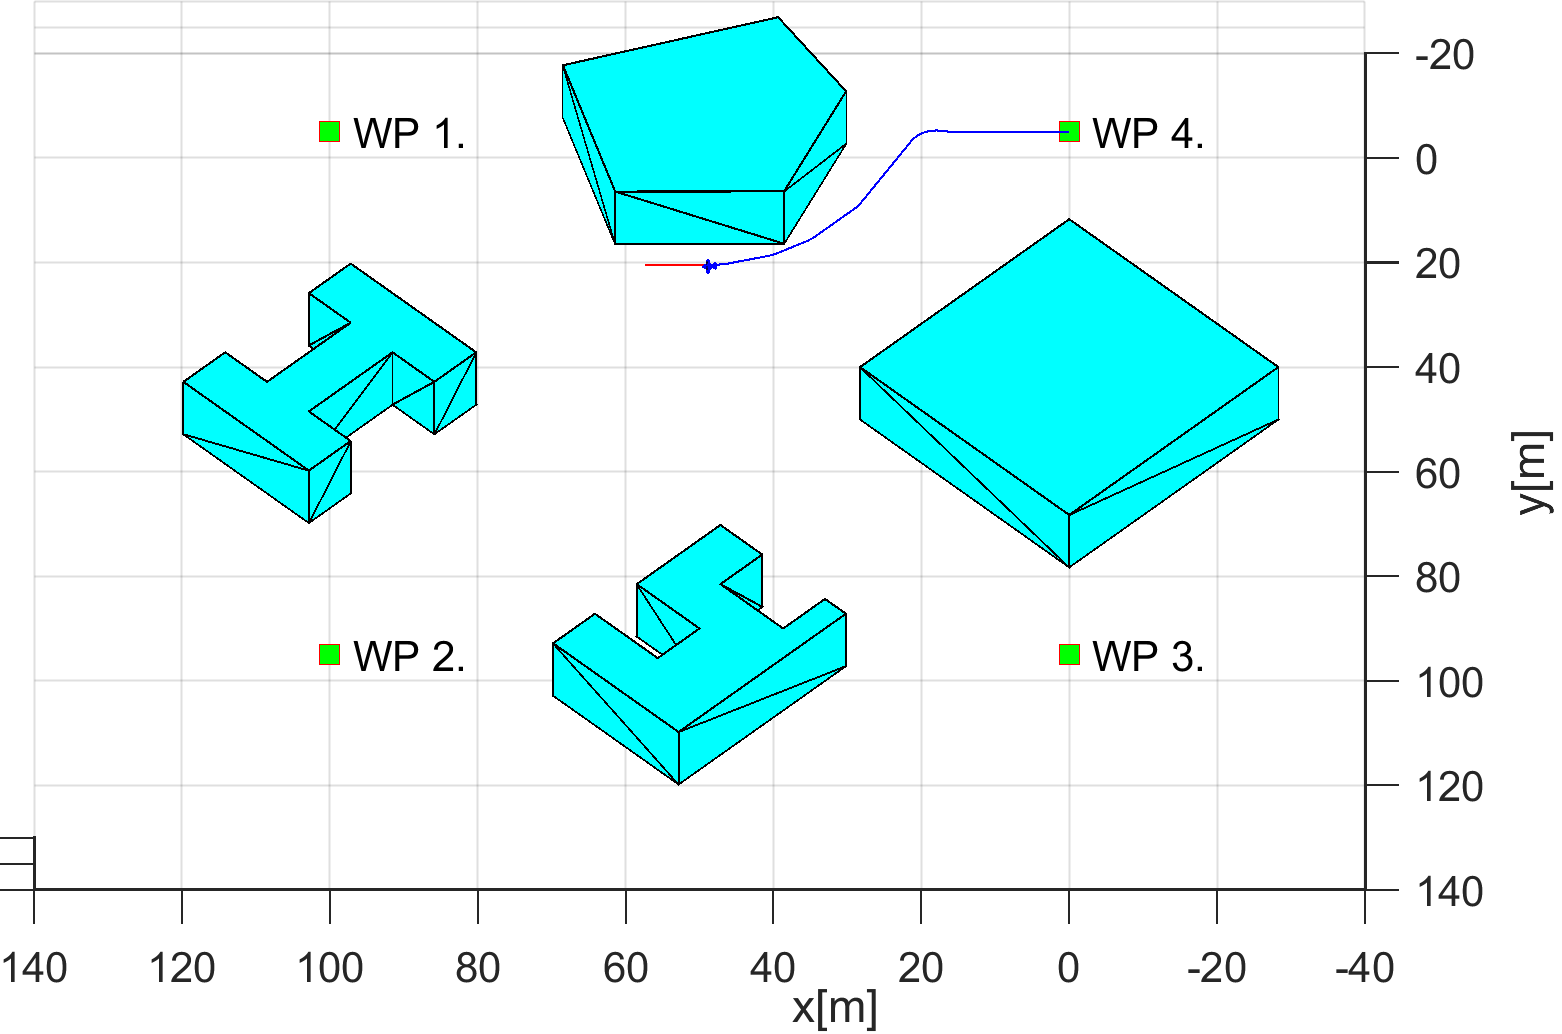
\includegraphics[width=0.9\linewidth]{\FIGDIR/NS001ConstraintsBuildingObstacle00061}
		\caption{$1^{st}$ building avoidance.}
		\label{fig:firstBuildingAvoidance}
	\end{subfigure}
	\begin{subfigure}{0.48\textwidth}
		\centering
		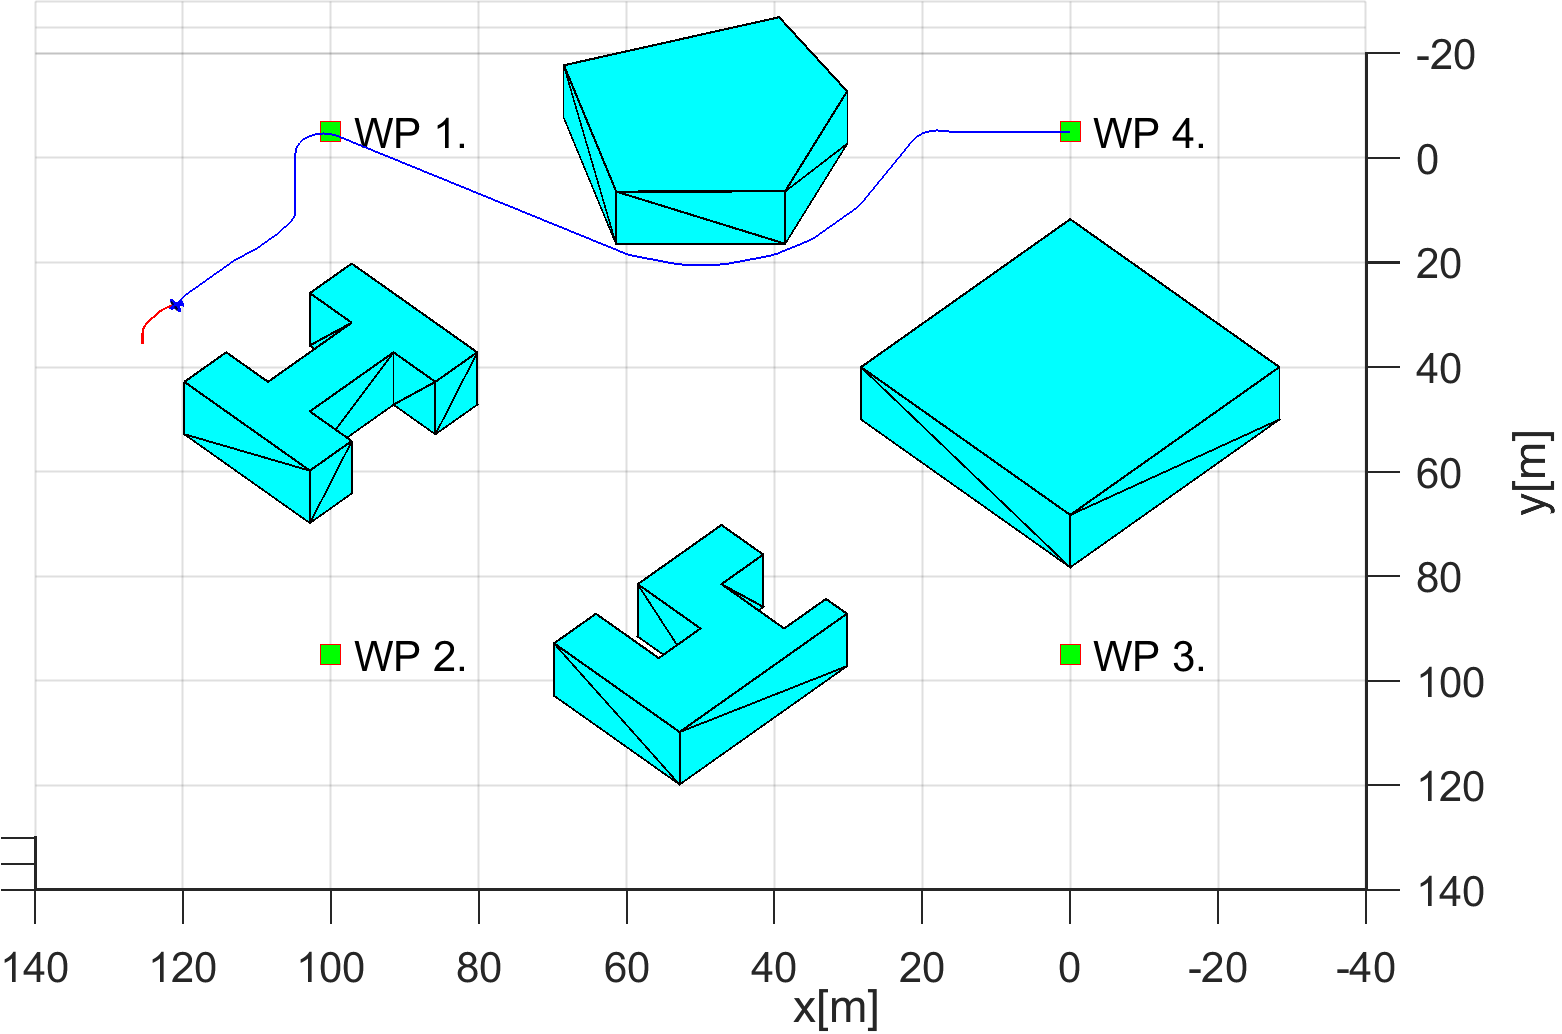
\includegraphics[width=0.9\linewidth]{\FIGDIR/NS002ConstraintsBuildingObstacles00161} 
		\caption{$1^{nd}$ building avoidance.}
		\label{fig:secondBuildingAvoidance}
	\end{subfigure}
	\\
	\begin{subfigure}{0.48\textwidth}
		\centering
		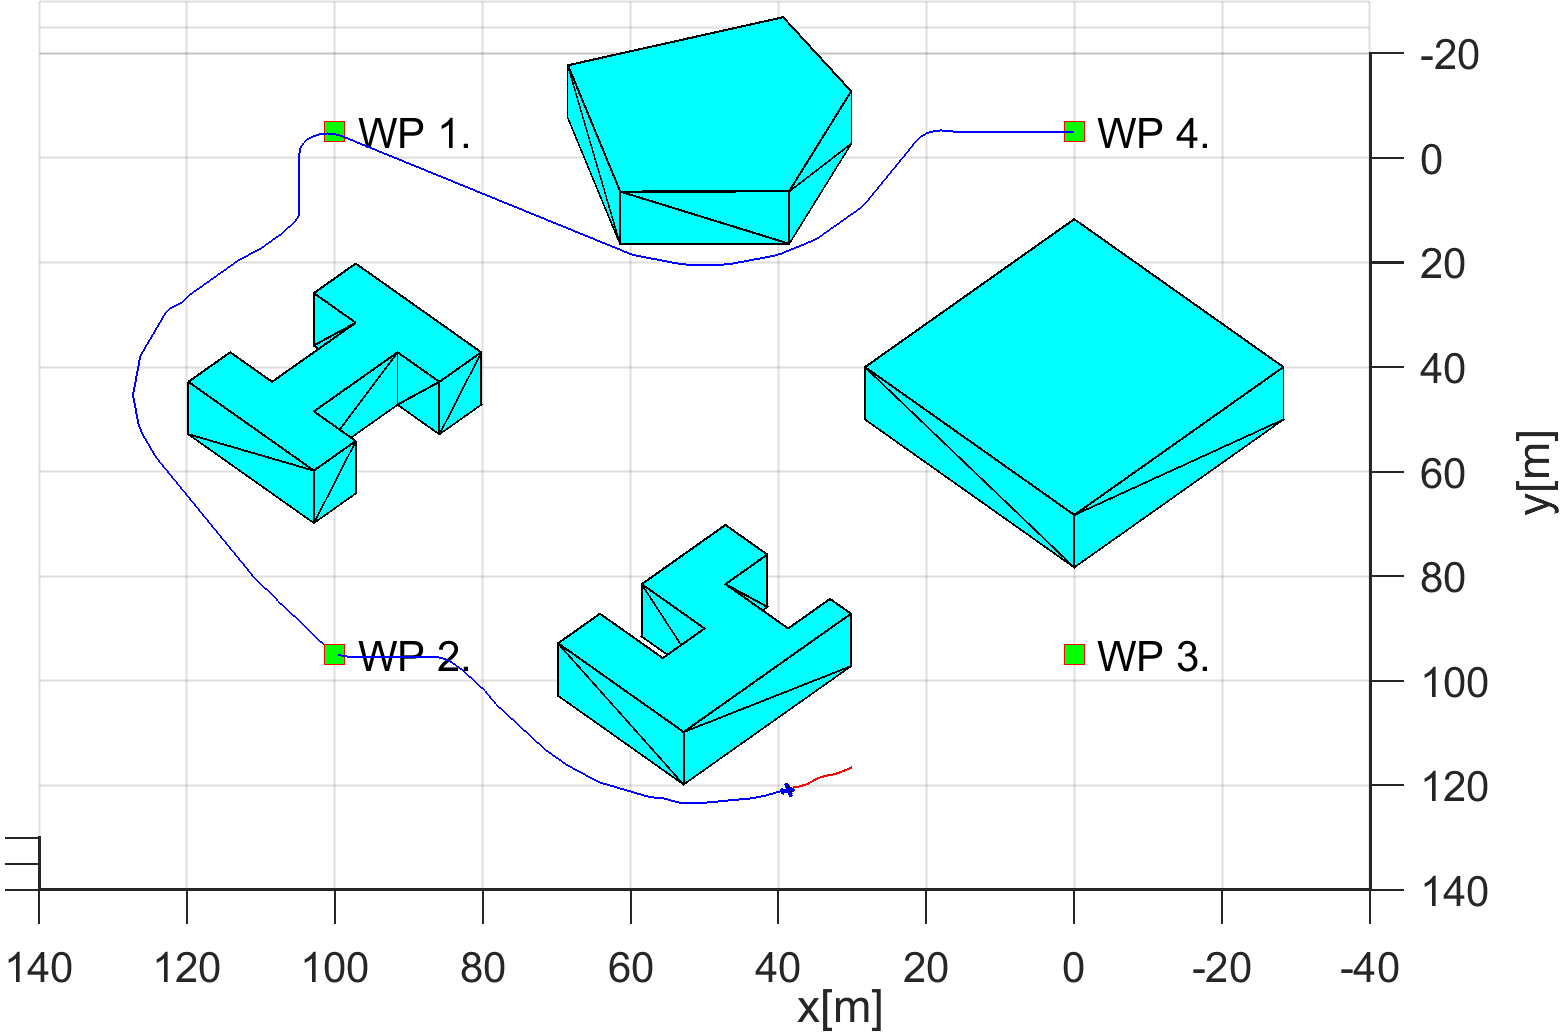
\includegraphics[width=0.9\linewidth]{\FIGDIR/NS003ConstraintsBuildingObstacles00311} 
		\caption{$3^{rd}$ building avoidance.}
		\label{fig:thirdBuidlingAvoidance}
	\end{subfigure}
	\begin{subfigure}{0.48\textwidth}
		\centering
		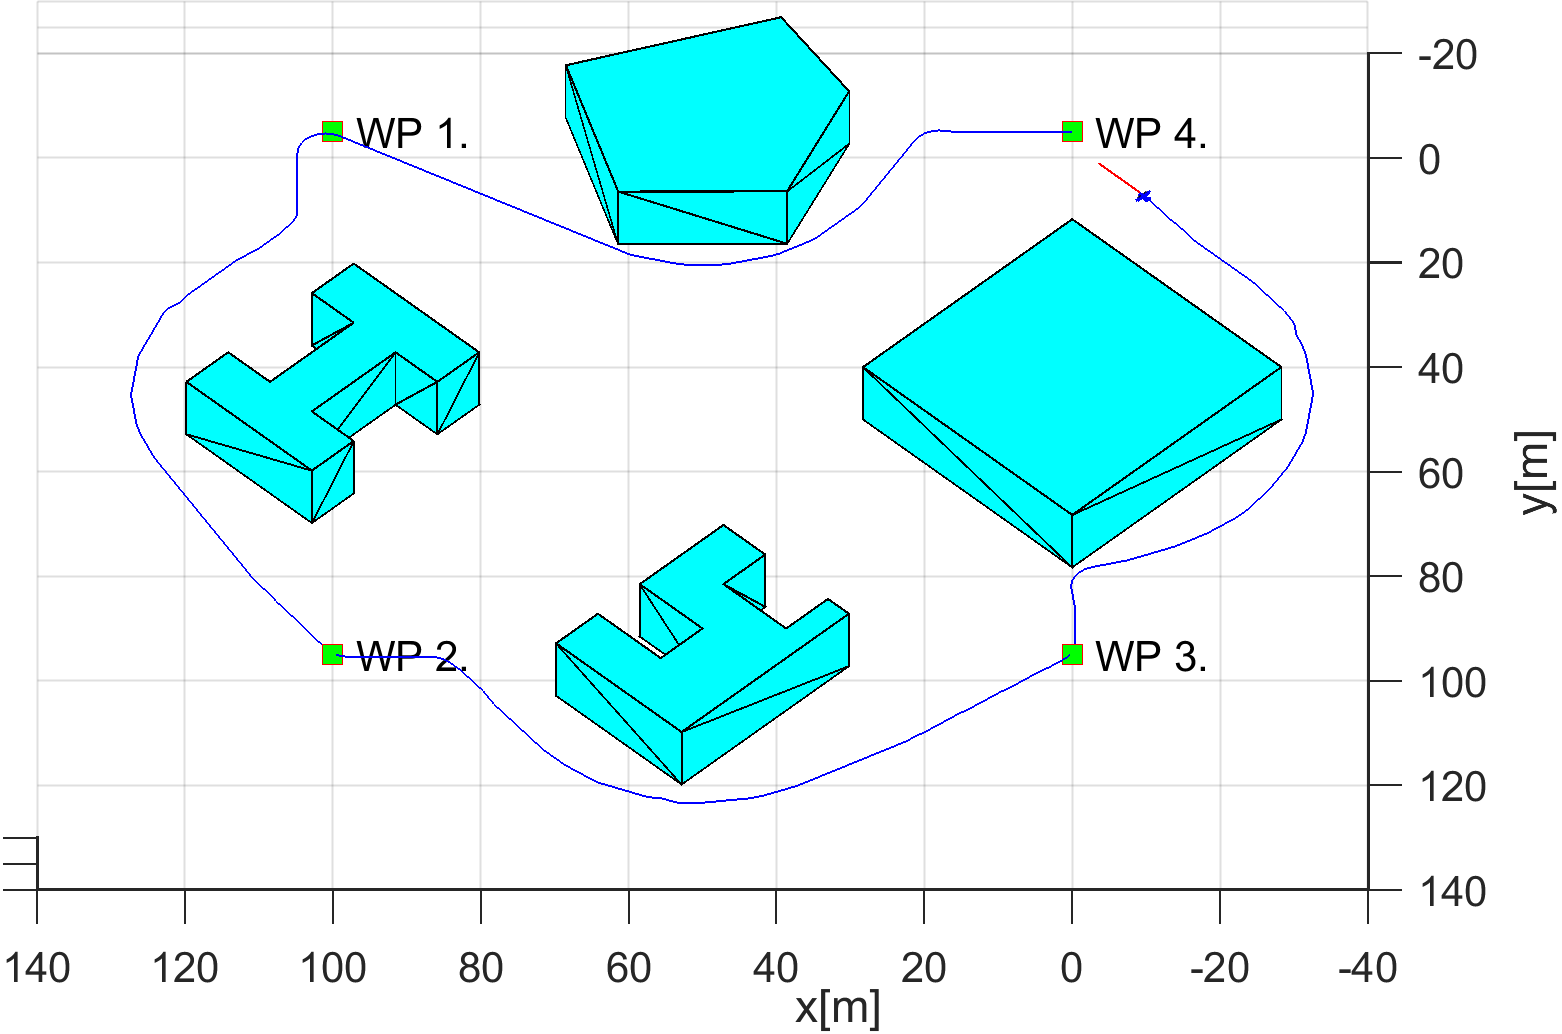
\includegraphics[width=0.9\linewidth]{\FIGDIR/NS004ConstraintsBuildingObstacles00470} 
		\caption{$4^{th}$ building avoidance.}
		\label{fig:fourthBuildingAvoidance}
	\end{subfigure}
	\caption{Test scenario for \emph{Building avoidance} (static ground obstacles). }
	\label{fig:testCaseBuildingAvoidanceSituation}
\end{figure}


\noindent\paragraph{Distance to Body/Safety Margin Evolution:} The distance of \emph{UAS} center to nearest obstacle (blue) does not broke a \emph{safety margin} (of closest obstacle (yellow)  nor \emph{body margin} of closest obstacle (red) as it can be seen in (fig. \ref{fig:testCaseBuildingAvoidancePerformance}). \emph{Acceptance condition} for \emph{algorithm mode switch} can be shown by UAS \emph{active avoidance of obstacles}.

\begin{note}
The \emph{body} and \emph{safety margins} are changing depending on \emph{UAS position and orientation}, is changing reflecting (tab. \ref{tab:obstacleSetBuildingAvoidance}) margins. 
\end{note}


\begin{figure}[H]
	\centering
	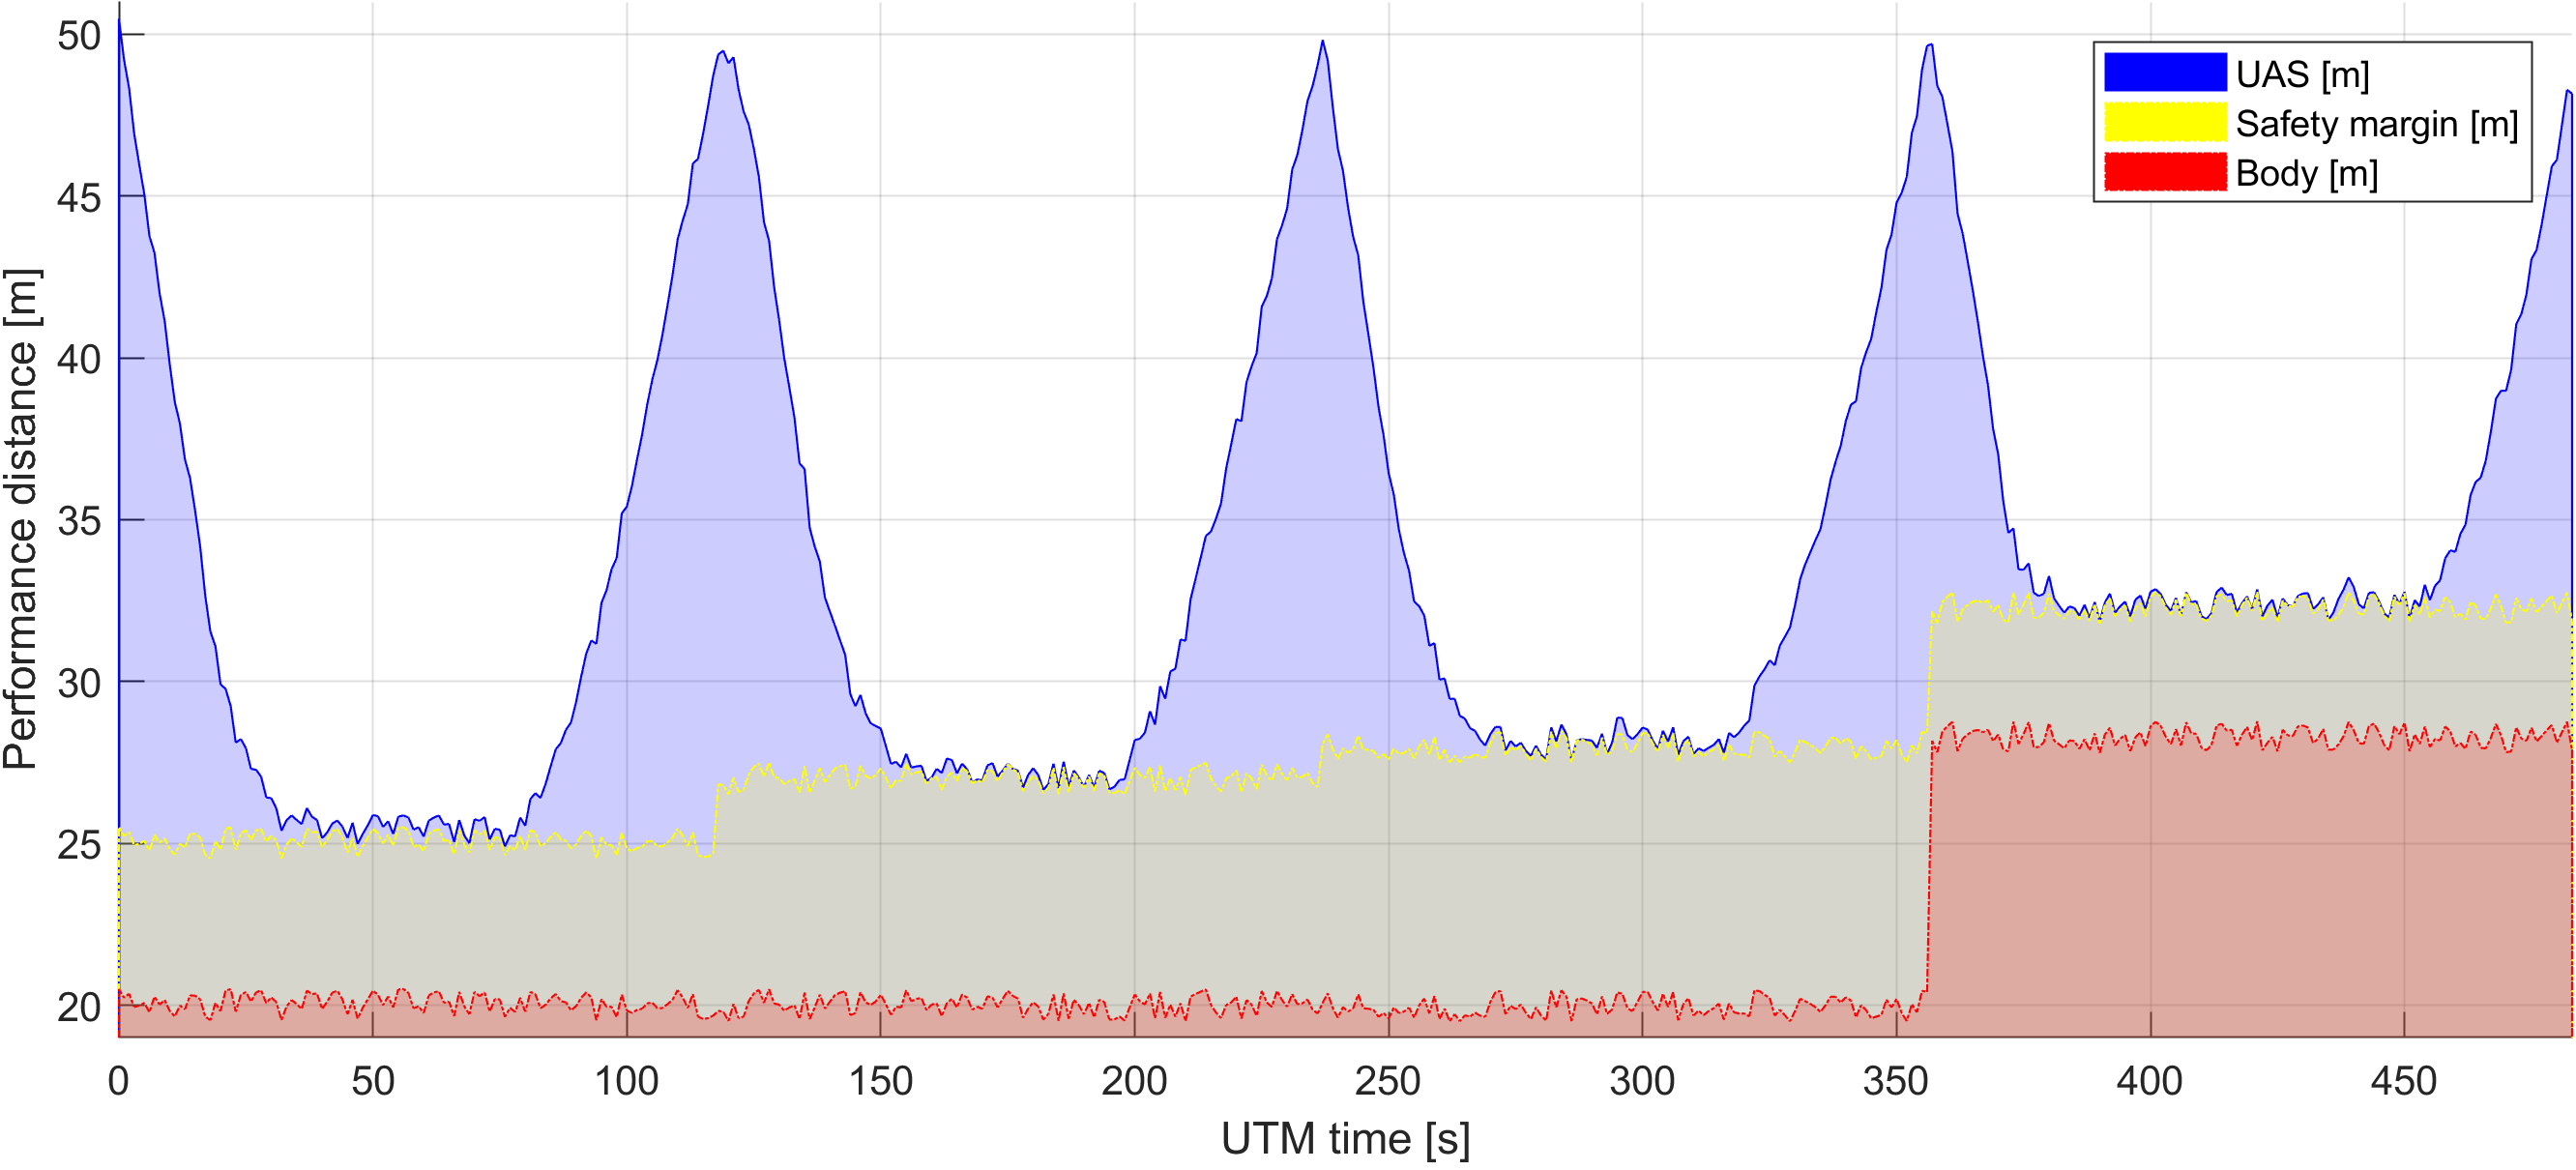
\includegraphics[width=0.8\linewidth]{\FIGDIR/NS005ConstraintsPolynomialBuildingObstaclesPerformance} 
	\caption{Distance to body/safety margin evolution for \emph{Building avoidance scenario}.}
	\label{fig:testCaseBuildingAvoidancePerformance}
\end{figure}


\noindent\paragraph{Distance to Body/Safety Margin Peaks:} Minimal distance to \emph{safety margin} is $0.69$ $m$. The \emph{minimal distance to obstacle body} is $4.69$ $m$ which is more than sufficient for tested UAS type. \emph{Safety margin acceptance criteria} have been achieved, because minimal distance is greater than zero. The minimal \emph{body margin distance} is $4.69$ $m$ for obstacle no. $4$ (tab. \ref{tab:obstacleSetBuildingAvoidance}).

\begin{table}[H]
	\centering
	\begin{tabular}{c|c||c}
	\multicolumn{2}{c||}{Parameter} & UAS 1 \\\hline\hline
	\multirow{2}{*}{safety margin distance} & min & 0.69  \\\cline{2-3}
											& max & 24.98 \\\hline
	\multirow{2}{*}{body margin distance}   & min & 4.69  \\\cline{2-3}
											& max & 29.98 
	\end{tabular}
	\caption{Distance to Body/Satety Margin Peaks for \emph{Building avoidance scenario}.}
	\label{tab:testCaseBuildingAvoidanceSafetyAndBodyMarginDistances}
\end{table}

\noindent\paragraph{Path Tracking Performance:} Reference path (green dashed line) is given as direct interconnection between waypoints (green numbered square).  The real trajectory (blue solid line) is split into its XYZ components. \emph{All mission waypoints} (fig. \ref{fig:testCaseBuildingAvoidancePathTracking}) have been reached in given order. There are some deviations on $X-Y$ horizontal axes, while the UAS was in the \emph{avoidance mode}.

\begin{figure}[H]
	\centering
	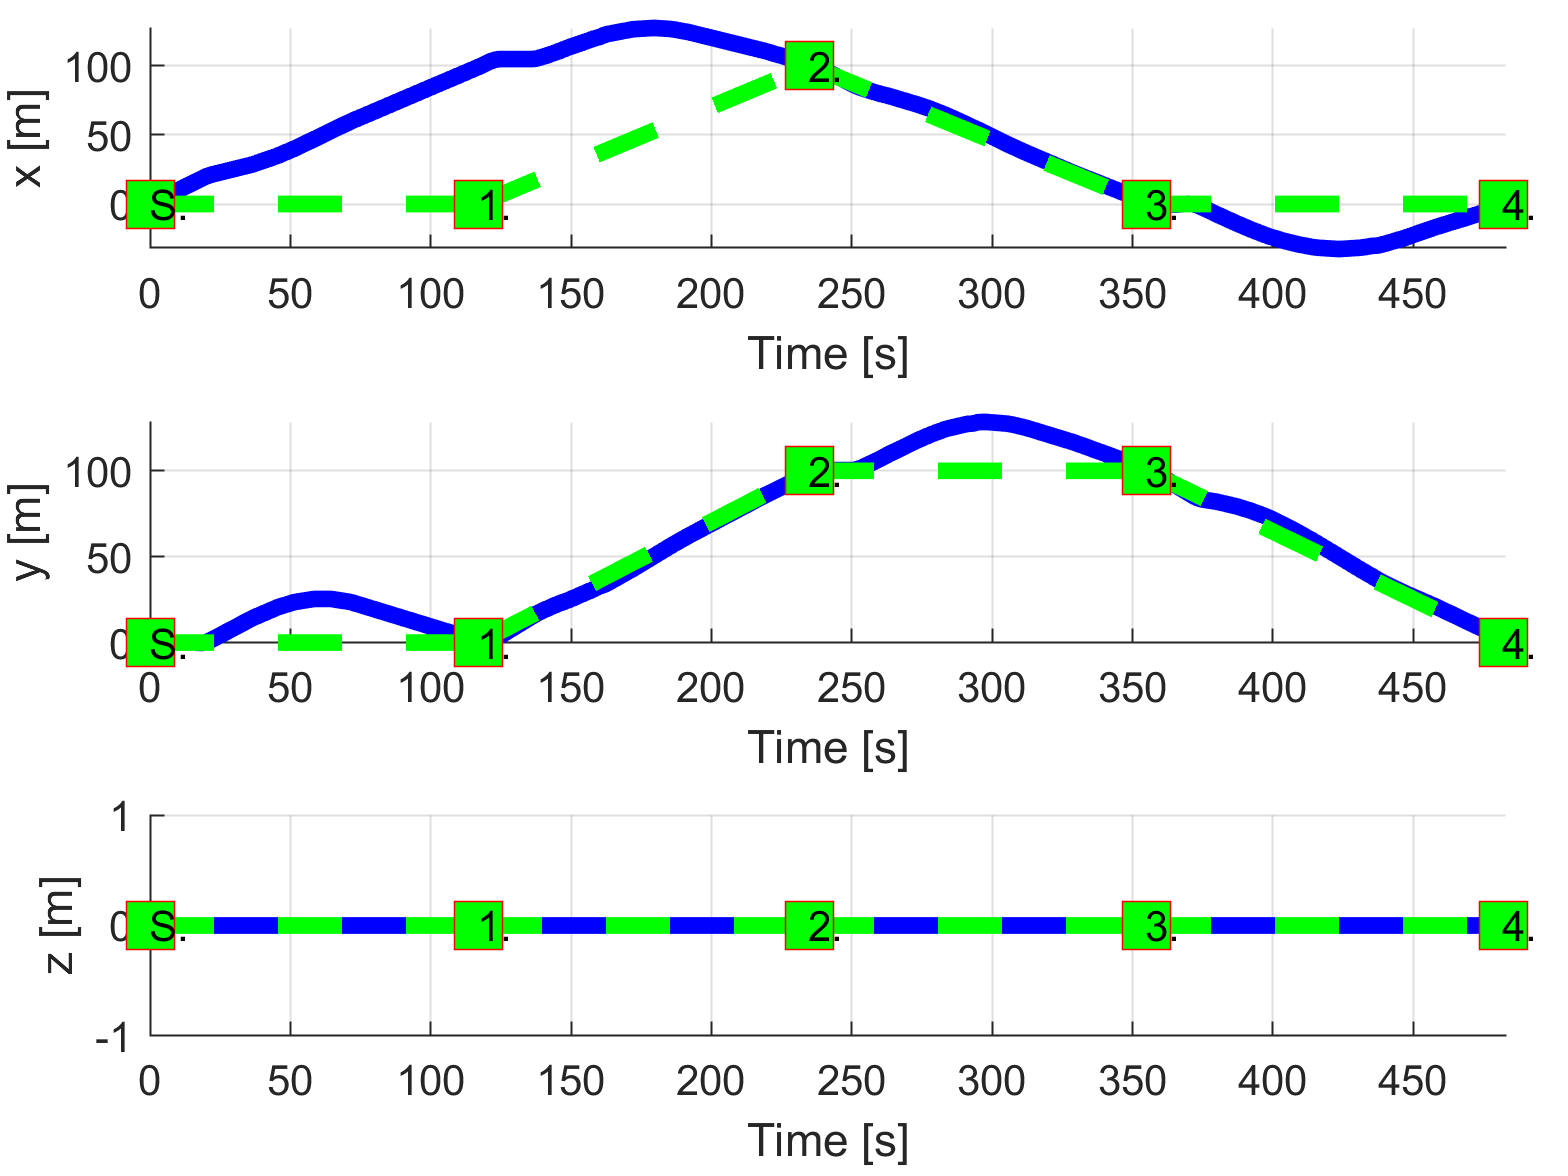
\includegraphics[width=0.55\linewidth]{\FIGDIR/NS006ConstraintsPolynomialBuildingPathFollowing} 
	\caption{\emph{Building avoidance} path tracking.}
	\label{fig:testCaseBuildingAvoidancePathTracking}
\end{figure}



\noindent\paragraph{Path Tracking Deviations:} Deviations (tab. \ref{tab:pathTrackingParametersForBuildingAvoidance}) from \emph{reference trajectory} are in expected ranges considering \emph{mission plan} (tab. \ref{tab:missionSetupForBuildingAvoidanceScenario}) and \emph{obstacle properties} (tab. \ref{tab:obstacleSetBuildingAvoidance}).
\begin{table}[H]
	\centering
	\begin{tabular}{c||c|c|c|c}
		\multirow{2}{*}{Param.} & \multicolumn{4}{c}{UAS 1} \\\cline{2-5}
						& $\mathscr{WP}_1$  & $\mathscr{WP_2}$  & $\mathscr{WP}_3$  & $\mathscr{WP}_4$  \\\hline\hline
		  $\max |x|$    & 104      & 86      & 5.34       & 32.52 \\\hline
		  $\max |y|$    & 25.39      & 6.59       & 28.2      & 4.55 \\\hline
		  $\max |z|$    & 0      & 0      &   0    & 0 \\\hline
		  $\max dist.$  & 107.05       & 86.2      & 28.7       & 32.84 \\
	\end{tabular}
	\caption{Path tracking for properties \emph{Building avoidance}.}
	\label{tab:pathTrackingParametersForBuildingAvoidance}
\end{table}
  


